\documentclass[]{beamer}
% Class options include: notes, notesonly, handout, trans,
%                        hidesubsections, shadesubsections,
%                        inrow, blue, red, grey, brown

% Theme for beamer presentation.
\usepackage{tabularx}
\usepackage{beamerthemesplit} 
% Other themes include: beamerthemebars, beamerthemelined, 
%                       beamerthemetree, beamerthemetreebars  

%\usepackage{beamerthemebars}

\title{LDPC Decoder Implementation using NoC}    % Enter your title between curly braces
\author{Shaishav Yogeshkumar Shah (133070050)}                 % Enter your name between curly braces
\institute{Supervisor: Prof. Sachin B. Patkar,\\
PhD Guide: Pinalkumar Engineer.\\
Dept. of EE,\\
IIT Bombay}      % Enter your institute name between curly braces
\date{\today}                    % Enter the date or \today between curly braces

\begin{document}

% Creates title page of slide show using above information
\begin{frame}
  \titlepage
\end{frame}
\note{Talk for 30 minutes} % Add notes to yourself that will be displayed when
                           % typeset with the notes or notesonly class options


\begin{frame}
  \frametitle{Acknowledgement}
  \begin{center}
  \begin{itemize}
    \item  \textbf{Prof. Sachin B. Patkar Sir} for giving me opportunity to present this idea and
      his consistent suggestion.
    \item  \textbf{Pinal J. Engineer}, PhD student for his good attention, idea suggestion, feasibility 
    and troubleshooting..
    
    
  \end{itemize}
   
  \end{center}

  
  \end{frame}
\section[Outline]{}

% Creates table of contents slide incorporating
% all \section and \subsection commands
\begin{frame}
  \tableofcontents [hideallsubsections]
\end{frame}

%%%%%%%%% LDPC Introduction

\include {ldpc_intro}



%%%%%%%% NoC Introduction
\include {noc_intro}


%%%%%%%% LDPC 7x7 Implementation

\section{PG-LDPC Implementation on un-partitioned/partitioned NoC}

%%%%%%% Insert Tanner Graph diagram and its explanation
\subsection{Tanner Graph formation}
\begin{frame}
\frametitle{Tanner Graph for PG-LDPC (7,3)}   % Insert frame title between curly braces
\begin{columns}[c]
\column{2.5in}  % slides are 3in high by 5in wide
\begin{itemize}
	\item PG-LDPC (7,3) code which is obtained by Projective Geometry over $GF(2^{s}),\ s=1$.
	\item The degree of total bit-node and check-node is $2^{s} +1 =3$.
	\item In this design, 5 bit precision :1 bit for sign, 3 bit of integer precision and 1 bit of fraction precision
\end{itemize} 

\column{2.5in}
\begin{center}
  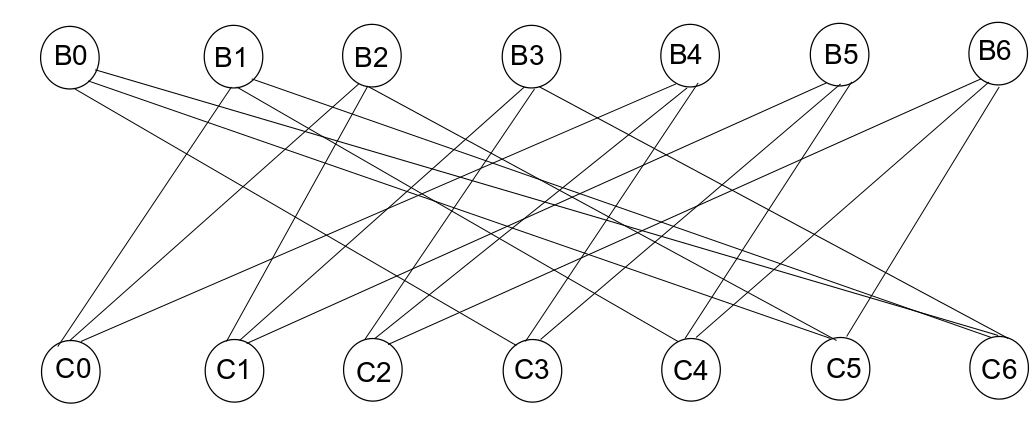
\includegraphics[scale=0.2]{./diagram/tanner_graph}
  Bn: Bit node n\\
  Cn: Check Node n
  \end {center}
  \end{columns}
\end{frame}


\begin {frame}
    \frametitle{How LDPC works?}
	  \begin{enumerate}
	  \item Initialize all bit nodes by Log Likelihood Ratio.
	  \item LLR propagates from bit nodes to check nodes via edges.
	  \item Check node performs computation.
	  \item Check node sends the computed LLR back to Bit node via edges.
	  \item Bit node checks whether the minimum required error is achieved or not.
	  \item If yes, sends the decoded data out, or else go to step(2).
	  \end{enumerate} 
\end {frame}

\subsection{Bit-Flipping Algorithm}
\begin{frame}
\frametitle{The Algorithm}   % Insert frame title between curly braces
A very simple explanation of bit-flipping algorithm is as follows
\begin{itemize}
	\item Check node bits are \textit{satisfied} if the sum of adjacent variable nodes is zero, \textit{unsatisfied} otherwise.
	\item Bit nodes flip the received value if the number of unsatisfied neighbours is larger than the number of satisfied neighbours.
\end{itemize}
\end{frame}



\subsection{PG-LDPC (7,3) Implementation using NoC}
\begin{frame}
\frametitle{System Implementation of PG-LDPC (7,3) using NoC}
\begin{columns}[c]
\column{2.2in}  % slides are 3in high by 5in wide
\begin{center}
Implementation on Mesh 4x4 un-partitioned NoC
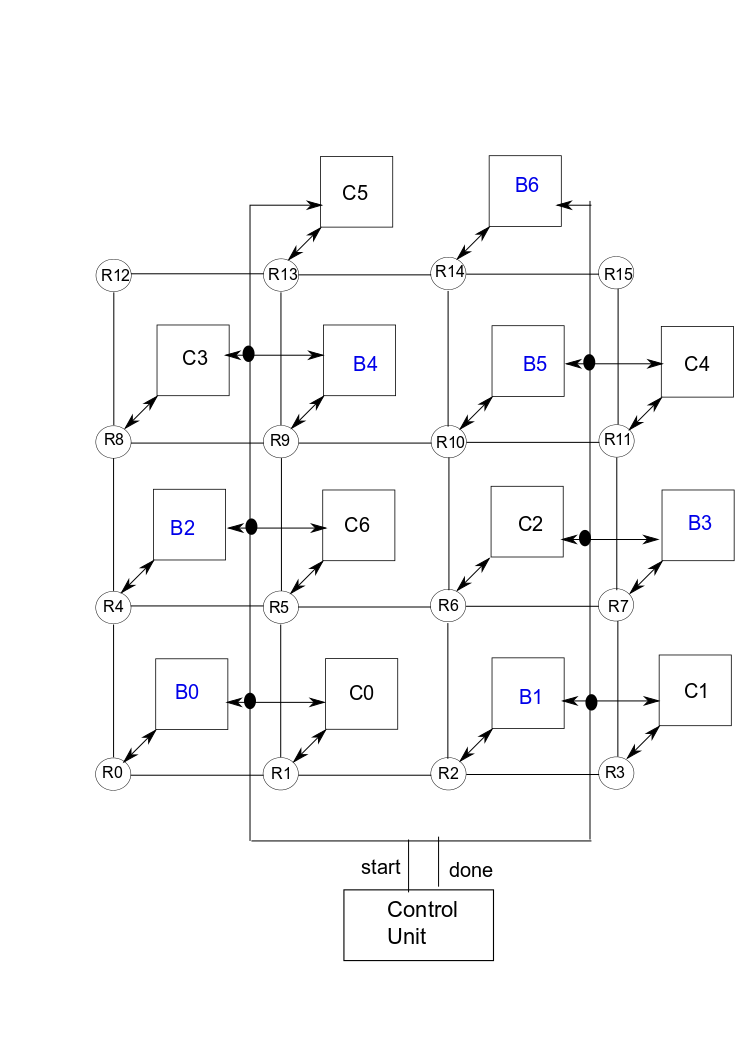
\includegraphics[scale=0.16]{./diagram/ldpc_7x7_noc_mesh_4x4}
\end{center}
\column{2.4in}
\begin{center}
Implementation on Mesh 4x4 partitioned NoC
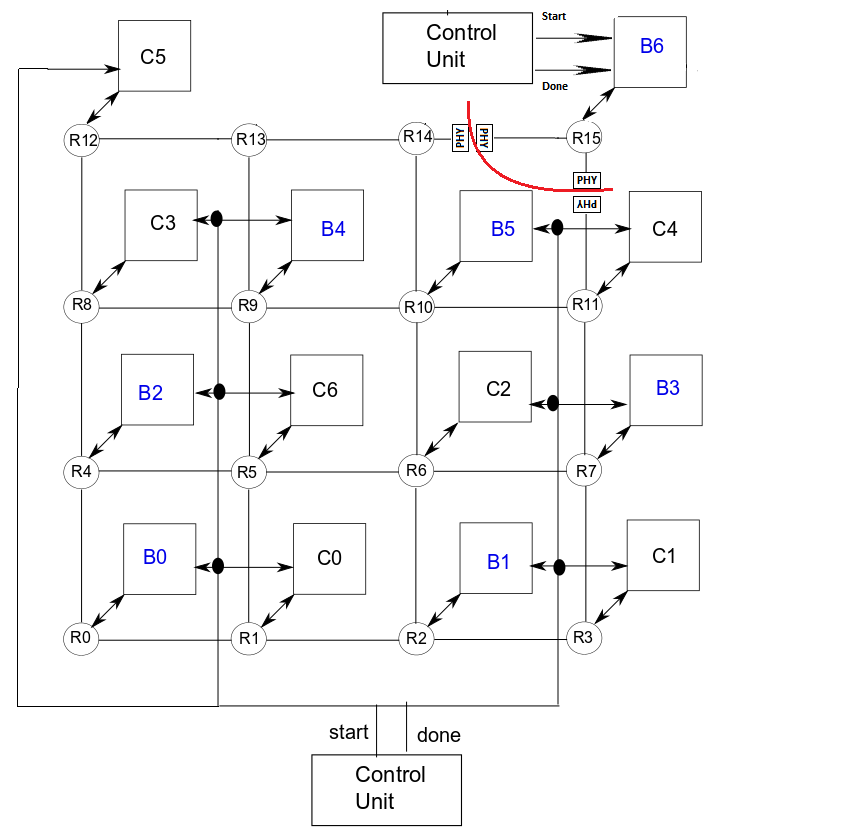
\includegraphics[scale=0.18]{./figs/Partitioned4X4Mesh}
\end{center}
\end{columns} 
\end{frame}

\subsection{Results and Comparison}
\begin {frame}
\frametitle {LDPC over NoC Flit Structure}
\begin{center}
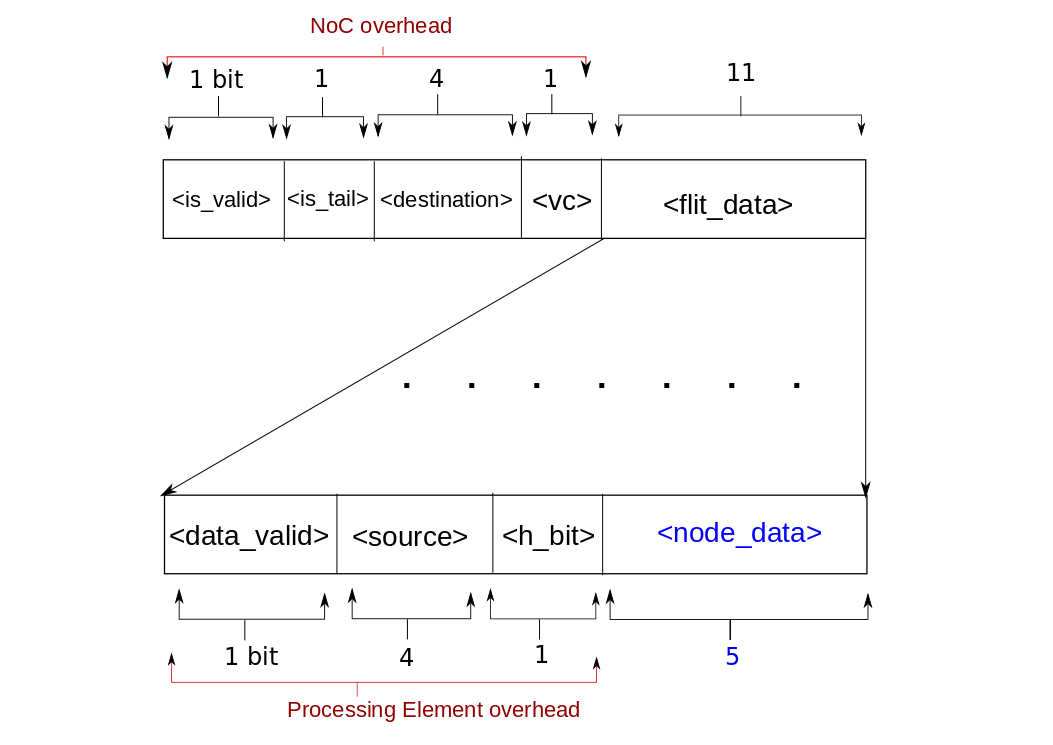
\includegraphics[scale=0.22]{./diagram/flit_structure_ldpc_7x7}
\end{center}

\end {frame}

\begin{frame}
\frametitle{Result comparison of Implementation of PG-LDPC(7,3) on un-partitioned NoC and partitioned NoC}
\begin{table} [scale=0.6]
\begin{center}
\resizebox{\textwidth}{!}
{\begin{tabular}{||c || c| c ||} \hline
Parameters 			      	& LDPC on 4$\times$4      	& LDPC on 4$\times$4 	\\ [0.5ex]
					& Mesh un-partitioned NoC 	& Mesh partitioned NoC  \\ \hline
Clock-cycle (1 iteration) 	      	& 18 				& 18+12\footnotemark	\\ \hline
Clock-cycle (n iteration) 	      	& 18 				& 18+12\footnotemark 	\\ \hline
Total cycle for n complete iteration 	& 18 + (n-1)$\times$12 		& (18 + (n-1)$\times$12) +12 \\ \hline
\end{tabular}}
\end{center}
\end{table}
\begin{center}
$Data Rate = \frac {Maximum\ frequency \times Data-width }{Nos\ of\ Iteration \times Nos\ of\ clock\ cycles} $.\\
\end {center}
\tiny
\textit{1,2:Whenever any data sent or received to or from partitioned node in this case for flit sent or received from bit node 15, additional 12 clock cycles is needed for the expected data to be received.}
\end{frame}

\begin{frame}
\frametitle{Performance Comparison and Resource Utilization for Altera :EP4CE22F17C6} 
\tiny
\begin{table} [scale=0.6]
\begin{center}
{\begin{tabular}{|| c || c | c | c ||}
\hline
				& Available  	& LDPC $7\times7$ Un-   & LDPC $7\times7$ 			\\ 
				& Resources  	& Partitioned      	& Partitioned Mesh 				\\
				&		& Mesh $4\times4$ NoC 	& $4\times4$ NoC				\\ \hline
	Number of		& 22,320     	& 9,840      	      	& 15,771 (71\%) (Part1) 			\\ 
	Logic Elements		&		& (44\%)		& 2,291  (10\%) (Part2)				\\ \hline
	Number of 		& 22,320     	& 6,651	              	& 11,113 (50\%) (Part1)				\\ 
	Logic Registers		&		& (30\%) 	      	& 1,787  (8 \%) (Part2)				\\ \hline
	Maximum Operating	& -          	& 36.27 MHz           	& 23.99 MHz 	(Part1)				\\  
	Frequency		&            	&                     	& 85.49 MHz	(Part2)				\\ \hline
	Number of clock		& -          	& 18                  	& 18 + 12(Part1)\footnotemark		\\ 
	cycles			&		&			& 18 + 12(Part2)\footnotemark		\\ \hline
	Data Rate		& -		& 36.27 Mbps		& 14.5 Mbps      				\\ \hline
\end{tabular}}
\end{center}
\end{table}

\tiny
\textit{1,2:Whenever any data sent or received to or from partitioned node in this case for flit sent or received from bit node 15, additional 12 clock cycles is needed for the expected data to be received.}
\end{frame}


  
  
  





%%%%%%%% LDPC 73x73 Implementation
\include {ldpc_73x73_noc}


%%%%%%%%%%%%%5 Conclusion and References
\section{Summary, Conclusion and Future Work}
\subsection{Summary}
\begin{frame}
\frametitle {Summary and Conclusion of work done}
\begin {center}
\begin{itemize}
\item NoC has been used as a data routing medium, which takes care of routing congestion
\item NoC partitioning will help isolating application node from the communication infrastructure
\item NoC integration with High speed serial Aurora Core very useful for Multi FPGA implementation
\item Quasi-SERDES module between routers of partitioned NoC is a viable alternate
\item Automation of NoC partitioning with inter-chip communication link integration using python scripts reduces the manual work tremendously
\end {itemize}
\end{center}
\end {frame}


\begin {frame}
\frametitle {Summary and Conclusion of work done (contd.)}
\begin {center}
\begin {itemize}
\item LDPC has a complex interconnect network, partitioned NoC can be used for data routing in Multi FPGA implementation
\item Bezier interpolation tested using DE0-Nano and Raspberry Pi working at 50 MHz converges in 0.161 seconds
\item Raspberry Pi can be used as FPGA/CPLD JTAG configuration (tested) and debugging platform (not tested)
\item FPGA/CPLD (Krypton board designed at WEL lab) can be configured using Raspberry Pi (tested), this is a suitable choice for remote lab set-up
\item Raspberry Pi interfacing with FPGA presents a viable software hardware co-design platform
\end {itemize}
\end{center}

\normalsize
\end {frame}

\subsection{Future Work}
\begin{frame}
\frametitle {Future Work}
\begin {center}
\begin {itemize}
\item Design of a scalable and a repeatable block style design of FPGA PCB for Multi-FPGA NoC implementation
\item A simple PCB design shown below which could be repeated to create n$\times$n Mesh of FPGA Network-of-Chips shown in the next slide
\end {itemize}
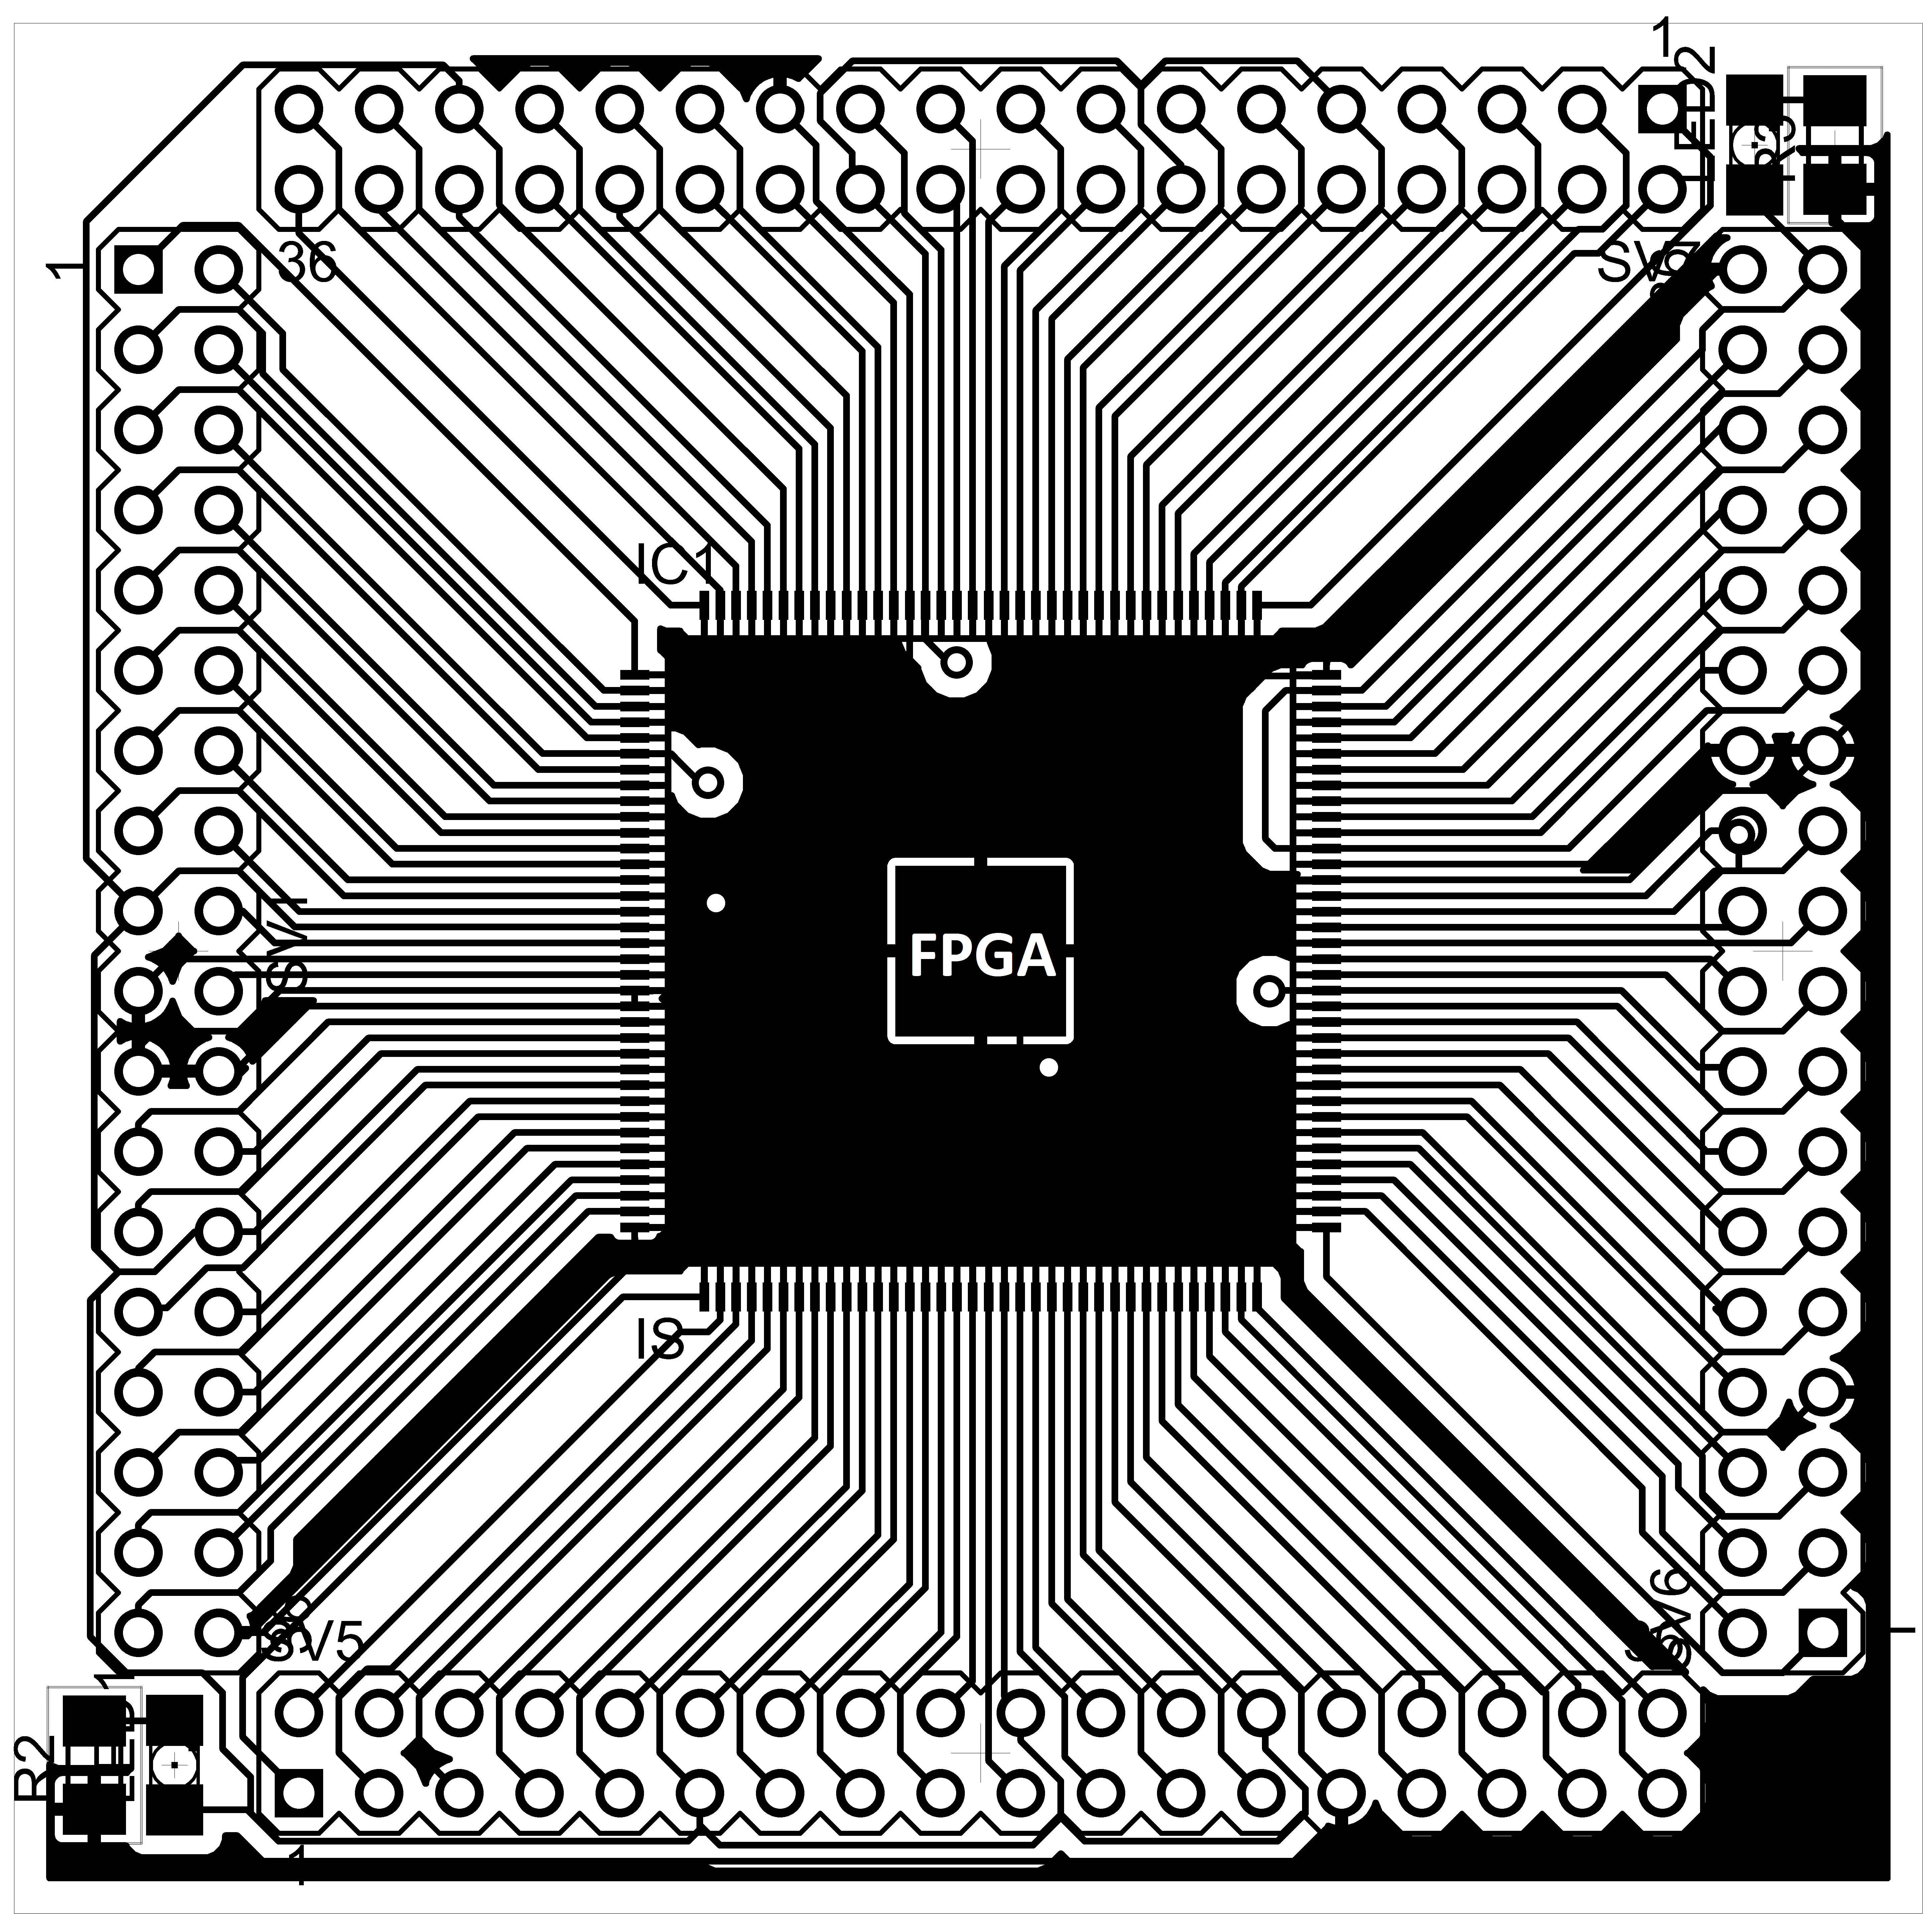
\includegraphics[scale=0.5]{./figs/BasicPCB}
\end {center}
\end{frame}

\begin{frame}
\begin {center}
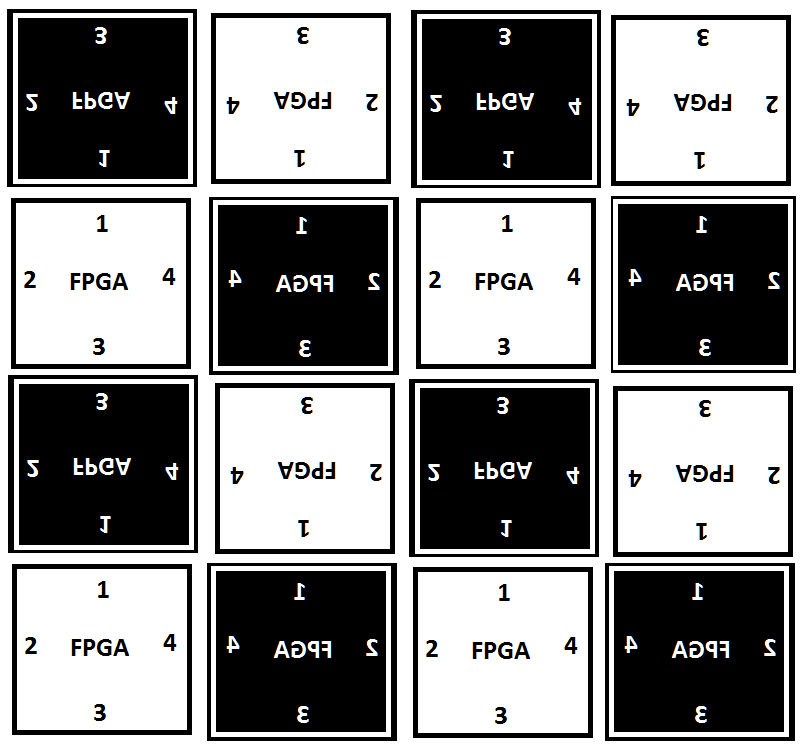
\includegraphics[scale=0.3]{./figs/MultiFPGANoC}
\end {center}
\end{frame}


\begin{frame}
\begin{center}
Thank You 
\end{center}

\end{frame}


	     % typeset with the notes or notesonly class options

\end{document}
